\documentclass[12pt,a4paper]{article}

% === Packages ===
\usepackage[utf8]{inputenc}
\usepackage[T1]{fontenc}
\usepackage{amsmath,amssymb,amsfonts,amsthm}
\usepackage{booktabs}
\usepackage{graphicx}
\usepackage{geometry}
\usepackage{array}
\usepackage{float}
\usepackage{xcolor}
\usepackage{enumitem}
\usepackage{hyperref}
\geometry{margin=1in}
\graphicspath{{./paper_figures/}}

\begin{document}

% === Title ===
\title{\textbf{Future Service Rights in Aviation:}\\%
\large Carrier-Level Credit, Booking-Curve Pricing, and $t$-Copula Structuring}

\author{Research Team\\
\textit{Flight Finance Research Group}}

\date{May 2026}
\maketitle

\begin{abstract}
We develop a Future Service Rights (FSR) securitization structure for commercial aviation. Unlike prior service-capacity securitization involving thousands of small independent operators, aviation concentrates default risk in 25 carriers. We address this through a reduced-form carrier credit model calibrated from the historical record of U.S. airline bankruptcies, a booking-curve pricing mechanism parameterized from the airfare dynamics literature, and a multivariate $t$-copula ($\nu=4$) with an empirically informed correlation matrix derived from airline equity returns (2021--2025). Using 97.3 million fare observations from the U.S. DOT DB1B survey, we construct a 69-route stratified pool across 11 carriers. Monte Carlo simulation (5,000 paths) with a standard bottom-up waterfall yields zero Senior expected loss---the maximum pool loss of 15.6\% never breaches the 35\% credit enhancement protecting the Senior tranche, implying a Moody's-equivalent rating of Aaa--Aa. Copula sensitivity analysis confirms this result across Gaussian, $t(6)$, and $t(4)$ specifications. The discount rate ($r_0 = 8\%$, based on airline industry WACC) is subjected to sensitivity analysis across $r_0 \in [4\%, 12\%]$; the Senior rating is robust throughout. Carrier-type-specific stress testing confirms investment-grade resilience through Systemic Shock scenarios. The booking-curve parameter~$\beta$ cannot be calibrated from the DB1B data; we show that user savings are determined by the discount rate and issue discount under our pricing specification, not by $\beta$, and report full sensitivity. The structure creates quadripartite value: users save 19\% versus last-minute booking (weighted ROI 16.4\%), carriers convert variable revenue to guaranteed upfront cash (\$1.69M at +1.5\% vs.\ spot), the platform earns 11.6\% ROI as market-maker, and Senior investors receive 5.50\% net yield with zero expected loss. We further model carrier secondary-market buyback---a mechanism with no analog in traditional airline finance---where carriers repurchase their own time-rights below 82\% of issue price, providing an implicit price floor for investors while capturing an additional 0.9\% of issue revenue. We conclude that flight capacity meets the credit quality threshold for standalone FSR securitization, with the Senior tranche benefiting from a substantial subordination buffer and incentive-aligned carrier participation.
\end{abstract}

% ============================================================
\section{Introduction}
% ============================================================

The global commercial aviation industry transports over 4 billion passengers annually, generating approximately \$900 billion in revenue. Yet the market for forward flight capacity remains primitive: a seat on a June 15 departure has economic value today, but that value is trapped. Airlines cannot sell that seat forward as a tradable instrument. Investors cannot gain exposure to flight demand without owning airline equity. Consumers cannot lock in forward prices except through non-transferable advance-purchase tickets.

The Future Service Rights (FSR) framework introduced the concept of a Time-Right---a tokenized contingent claim on a service provider's future capacity---and demonstrated viability in the service sector \cite{fsr2026}. Extending this framework to aviation requires a fundamentally different credit architecture. Prior FSR work relied on a pool of thousands of independent properties with largely idiosyncratic default risk and a Gaussian copula. Aviation presents a contrasting topology: 102,279 origin-destination pairs served by only 25 carriers, with the top four holding 62.4\% of passenger volume. A single carrier's bankruptcy triggers simultaneous default across all of its pooled routes.

Table~\ref{tab:hotel_vs_flight} summarizes the key structural differences between hotel FSR and flight FSR that motivate our modeling choices.

\begin{table}[H]
\centering
\caption{Hotel FSR vs.\ Flight FSR — Structural Comparison}
\label{tab:hotel_vs_flight}
\begin{tabular}{lcc}
\toprule
\textbf{Dimension} & \textbf{Hotel FSR} & \textbf{Flight FSR (this paper)} \\
\midrule
Credit entity        & Individual hotel property & Individual carrier \\
Number of entities   & 16,257 (high granularity) & 25 (concentrated) \\
Default correlation  & Gaussian copula & $t$-copula ($\nu = 4$) \\
PD driver            & Price CV (Merton DD) & Historical bankruptcy frequency \\
Booking mechanism    & Spot-price convergence & Exponential booking curve \\
Maturity             & 36 months & 12 months \\
Tranche structure    & 68/20/8/4 & 65/20/10/5 \\
Senior subordination & 32\% & 35\% \\
Senior rating        & Aa-A (EL 0.16\%) & Aaa-Aa (EL 0 bps) \\
Max pool loss        & Not reported & 15.6\% \\
\bottomrule
\end{tabular}
\end{table}

This paper makes three contributions. First, we construct a reduced-form carrier credit model calibrated from the historical record of U.S. airline bankruptcies (2000--2025). The model separates operational volatility---fare coefficient of variation, driven by yield management and fare-class segmentation---from financial distress risk. Second, we introduce booking-curve pricing, replacing the spot-convergence mechanism used in prior FSR work. Third, we deploy a $t$-copula with $\nu = 4$ degrees of freedom, using an empirically informed correlation matrix derived from 5-year daily airline equity returns.

We calibrate the model using 97.3 million fare observations from the U.S. DOT DB1B survey (2022Q1--2025Q1). The resulting 69-route stratified pool yields a Senior tranche rated Aaa--Aa (EL 0 bps) under $t(4)$-copula simulation, protected by 35\% subordination that the maximum pool loss of 15.6\% never breaches. A full-period pessimistic calibration (2000--2025) increases the pool PD from 0.76\% to 1.15\%, and carrier-type-specific stress tests confirm investment-grade resilience. We conduct sensitivity analysis on the discount rate $r_0$, the issue discount $d$, and the booking-curve parameter $\beta$, identifying which results are model-driven and which are structural.

% ============================================================
\section{Data and Exploratory Analysis}
% ============================================================

\subsection{Data Source and Limitations}

We use the U.S. DOT DB1B Origin and Destination Survey (Market segment), a 10\% quarterly sample of all domestic U.S. airline tickets \cite{bts2025}, spanning 13 quarters (2022Q1--2025Q1): 97.3 million records, 102,279 unique origin-destination (OD) pairs, and 25 distinct carriers.

Two limitations are material. First, DB1B records tickets by travel quarter, not purchase date, preventing direct calibration of the booking curve (Section 4.3). Second, the 10\% sample introduces variance in route-level statistics; for thin routes near our 20-observation filter, sampling error inflates the observed fare CV. Pool weighting by passenger volume mitigates this by down-weighting thin routes. The median route in our pool has 145 observations.

\subsection{Key Structural Properties}

Two properties have first-order implications for FSR design.

\textbf{Extreme route concentration.} The top 1\% of routes (1,023 OD pairs) account for 50.3\% of passenger volume; the top 10\% capture 92.9\%. The route-level Gini coefficient is 0.91. This concentration is structural---hub-to-hub routes dominate---and implies unavoidable exposure to hub-specific disruptions.

\textbf{The competition paradox is reversed.} Monopoly routes exhibit mean fare CV of 0.52, while routes with 10+ carriers exhibit mean CV of 0.63. Additional competition increases within-route fare dispersion through fare-class proliferation. The direct implication: fare CV cannot serve as a primary default proxy in aviation, as it primarily reflects yield management sophistication rather than financial distress. Extreme fare CV values for small carriers (e.g., carrier 3M exhibits CV $\approx$ 19.5 across 1,198 routes) are clamped to $\pm 40\%$ of the median by the credit model's CV adjustment factor (Eq.~\ref{eq:cv_adj}), preventing data errors or tiny-carrier variance from contaminating the PD calibration.

\textbf{Carrier concentration.} The HHI is 1,160, with the top 4 carriers holding 62.4\% of volume. Table~\ref{tab:carriers} lists the 10 largest carriers.

\begin{table}[H]
\centering
\caption{Top 10 Carriers by Passenger Volume (2024 Q2)}
\label{tab:carriers}
\begin{tabular}{llrrrr}
\toprule
\textbf{Code} & \textbf{Carrier} & \textbf{Pax (M)} & \textbf{Share (\%)} & \textbf{Routes} & \textbf{Fare CV} \\
\midrule
WN & Southwest  & 41.6 & 21.9 & 10,517 & 0.552 \\
DL & Delta      & 28.5 & 15.0 & 37,404 & 0.754 \\
AA & American   & 26.2 & 13.8 & 47,701 & 0.782 \\
UA & United     & 22.5 & 11.8 & 41,351 & 0.829 \\
NK & Spirit     & 10.3 &  5.4 &  3,031 & 0.654 \\
B6 & JetBlue    &  9.0 &  4.7 &  5,032 & 0.844\footnotemark[1] \\
AS & Alaska     &  8.4 &  4.4 & 13,557 & 0.732 \\
OO & SkyWest    &  8.1 &  4.2 & 71,352 & 2.618 \\
F9 & Frontier   &  8.1 &  4.3 &  5,476 & 0.634 \\
G4 & Allegiant  &  5.4 &  2.8 &  1,384\footnotemark[2] & 0.598 \\
\bottomrule
\end{tabular}
\footnotetext[1]{B6's CV of 0.844 exceeds NK's 0.654 despite less aggressive yield management. This is attributable to B6's Northeast-focused network with high business-leisure fare mixing on premium transcontinental routes (JFK--LAX, JFK--SFO).}
\footnotetext[2]{G4's 1,384 routes reflect OD pairs served during 2024 Q2 specifically. G4 operates low-frequency (2--4 flights/week) seasonal leisure routes; the passenger-to-route ratio ($\sim$43 daily pax per route) is consistent with this model.}
\end{table}

SkyWest (OO) exhibits fare CV of 2.618, reflecting its role as a regional contract carrier under capacity purchase agreements (CPAs)---not elevated bankruptcy risk. This observation directly motivates our separation of operational volatility from credit risk.

% ============================================================
\section{Carrier Credit Model}
% ============================================================

\subsection{Design Principle}

In credit models where the operator \emph{is} the asset, price volatility can serve as a direct PD proxy. This approach fails for airlines because fare dispersion is dominated by yield management \cite{belobaba2015}. Delta's fare CV of 0.75 reflects revenue optimization, not financial distress.

We adopt a reduced-form, scorecard-based calibration with three components. The model does not explicitly incorporate fleet age, fuel hedging ratios, labor cost structure, or macro factor exposures (GDP, oil price). These factors are correlated with carrier type and market position---majors operate younger fleets, maintain active fuel hedging programs, and have greater capacity to absorb labor cost increases than LCCs or regionals---so the carrier-type classification and market-share adjustment in our model partially proxy for these omitted variables. A structural model incorporating balance-sheet data would capture them more directly, at the cost of the opacity introduced by airline asset-valuation complexity (see above).

\begin{enumerate}[label=(\roman*)]
    \item \textbf{Base default probability}---calibrated from historical bankruptcy frequency, differentiated by carrier type;
    \item \textbf{Market position adjustment}---larger carriers receive lower PDs;
    \item \textbf{Operational volatility adjustment}---fare CV provides a \textit{limited} modifier ($\pm 40\%$ range) to the base PD.
\end{enumerate}

This approach is deliberately simpler than a full Merton-style structural model. The Merton (1974) framework, as operationalized by Bharath and Shumway (2008) and the KMV model \cite{crosbie2003}, maps equity volatility to asset volatility and computes distance-to-default from balance-sheet data. Airline balance-sheet data is publicly available for all major carriers and could in principle support asset-value-based PD estimation. However, airline asset values are dominated by fleet valuation (which depends on secondary-market aircraft prices and lease structures) and intangible assets (slot rights, brand value, loyalty program databases), making the standard Merton mapping from equity volatility to asset volatility unreliable. Our reduced-form approach prioritizes transparency and historical calibration over structural complexity, at the cost of not incorporating forward-looking balance-sheet information.

\subsection{Base PD Calibration}

We calibrate base PDs from the complete record of U.S. passenger airline Chapter 11 filings (2000--2025). The post-consolidation era (2013+) exhibits zero major-carrier defaults among the Big 4 and Alaska over 12 years (60 carrier-years). Spirit Airlines' 2024 filing is the sole major-carrier event; Spirit continued operating throughout its restructuring.

We set base annual PDs: WN 0.10\% (never filed, 50+ years); DL, UA 0.30\% (19--23 years clean); AA 0.40\% (14+ years); AS 0.20\% (never filed); B6 1.50\%; NK 5.00\% (filed 2024, \textit{ex post}); F9 2.00\%; G4 1.20\%; HA 1.00\%; CPA regionals 0.80--1.50\%; unclassified 2.50\%.

\textbf{Statistical power caveat.} The post-2013 calibration rests on 60 carrier-years with zero defaults among major carriers. This is both a strength---the industry is demonstrably safer post-consolidation---and a fundamental statistical limitation. Under a Poisson model with zero observed events, the 95\% confidence upper bound for the annual default rate is approximately 3/60 $\approx$ 5.0\%. The 90\% upper bound is $\approx$ 3.6\%. This means the \textit{true} major-carrier PD could plausibly range from 0.1\% to 5\% and we cannot distinguish these values with the available data. Our calibrated PDs of 0.10--0.40\% represent a judgment that the post-consolidation era is structurally safer rather than statistically lucky, but we cannot prove this from the default record alone. This is an irreducible limitation that no amount of model sophistication can overcome---it is a data constraint, not a modeling choice.

Critically, \textbf{the Senior rating result does not depend on PD precision}. Table~\ref{tab:pd_robustness} demonstrates this directly: even at the 95\% Poisson upper bound (PD $\approx$ 5\%), the pool expected loss is approximately 5\% $\times$ 17.7\% LGD $\approx$ 0.89\%, against 35\% Senior subordination. The Senior attachment point is breached only when the pool PD exceeds approximately $35\% / 17.7\% \approx 198\%$, a physical impossibility. This bounding calculation reveals that the paper's headline finding rests not on the precision of the PD estimates but on the \textit{thickness of the subordination structure} relative to any plausible pool loss. A more precise PD estimate would shift the Equity and Junior expected losses but would not alter the Senior rating. We state this explicitly because it is the honest reason the result is robust: the 35\% buffer is simply too large relative to any plausible pool PD.

\begin{table}[H]
\centering
\caption{Senior Rating Robustness to PD Calibration Range}
\label{tab:pd_robustness}
\begin{tabular}{lccc}
\toprule
\textbf{PD Scenario} & \textbf{Pool PD} & \textbf{Pool EL (approx.)} & \textbf{Senior EL} \\
\midrule
Baseline (post-2013)         & 0.76\% & 0.13\% & 0 bps \\
Pessimistic (2000--2025)     & 1.15\% & 0.20\% & 0 bps \\
90\% Poisson upper bound     & 3.6\%  & 0.64\% & 0 bps \\
95\% Poisson upper bound     & 5.0\%  & 0.89\% & 0 bps \\
10$\times$ baseline (extreme)& 7.6\%  & 1.35\% & 0 bps \\
Breakeven for Senior         & 198\%  & 35.0\% & $>$0 bps \\
\bottomrule
\end{tabular}
\end{table}

The structural thickness argument has one vulnerability: it assumes LGD remains at its calibrated level (17.7\%) under extreme PD scenarios. A correlated PD-LGD regime---where defaults cluster during industry-wide crises and recovery rates simultaneously collapse---could produce pool losses higher than the PD $\times$ LGD product suggests. We address this through historically calibrated stress tests (Section 5.3) that simultaneously increase PDs and LGDs. Under 9/11-scale and 2008-scale stress, the Senior EL remains zero; only COVID-scale stress (15$\times$ major PD, with LGD rising to 1.6$\times$) breaches the Senior at 329 bps. The combination of structural thickness and stress-test confirmation provides a more robust argument than PD precision alone could offer.

\textbf{Pessimistic calibration.} To address potential survivorship bias in the post-2013 window, we also calibrate using 2000--2025, which includes 6 major-carrier bankruptcies. Under this window, the pool-weighted PD increases from 0.76\% to 1.15\%. We use the post-2013 window as baseline and report the pessimistic calibration as a robustness bound. The structural argument for the narrower window---industry consolidation enabled capacity discipline and ancillary revenue growth \cite{borenstein2011}---is acknowledged as a judgment call, and the pessimistic bound provides a conservative alternative.

\subsection{Size and Volatility Adjustments}

The size adjustment factor is:
\begin{equation}
s_i = \frac{1}{\max(0.4, \; 1.0 + 0.4 \cdot \ln(m_i \cdot 100))}
\label{eq:size_adj}
\end{equation}
where $m_i$ is market share. For Southwest ($m_i = 0.219$), $s_i = 0.45$. The volatility adjustment is:
\begin{equation}
v_i = 1.0 + \text{clip}\left( \frac{cv_i - \bar{cv}}{\bar{cv}}, \; -0.4, \; 0.4 \right)
\label{eq:cv_adj}
\end{equation}
where $\bar{cv} = 0.65$. The final PD is $\text{PD}_i = \text{PD}_i^{\text{base}} \cdot s_i \cdot v_i$, floored at 0.30\% and capped at 35\%.

\subsection{LGD Calibration}

Airline Chapter 11 is restructuring: operations continue, flights depart, tickets are honored. In liquidation, DOT regulations require ticket refunds, and competitors offer rescue fares. We calibrate LGD: majors 15\%, LCCs 30\%, CPA regionals 10\%, unclassified 25\%. Pool-weighted LGD is 17.7\%. For regional carriers under CPAs, the credit structure involves two layers---the regional's own health and the partner's willingness to assume CPA contracts---which our single-layer model captures conservatively.

\subsection{Results}

Table~\ref{tab:credit_results} presents calibrated metrics. Table~\ref{tab:rating_map} provides the EL-to-rating mapping.

\begin{table}[H]
\centering
\caption{Calibrated Carrier Credit Metrics}
\label{tab:credit_results}
\begin{tabular}{llrrrrrr}
\toprule
\textbf{Code} & \textbf{Type} & \textbf{Base PD} & \textbf{Size Adj.} & \textbf{CV Adj.} & \textbf{Cal. PD} & \textbf{LGD} & \textbf{Rating} \\
\midrule
WN & Major & 0.10\% & 0.45 & 0.85 & 0.30\% & 15\% & A \\
DL & Major & 0.30\% & 0.48 & 1.16 & 0.30\% & 15\% & A \\
AA & Major & 0.40\% & 0.49 & 1.20 & 0.30\% & 15\% & A \\
UA & Major & 0.30\% & 0.50 & 1.28 & 0.30\% & 15\% & A \\
AS & Major & 0.20\% & 0.63 & 1.13 & 0.30\% & 15\% & A \\
B6 & LCC   & 1.50\% & 0.62 & 1.30 & 1.20\% & 30\% & Ba \\
NK & LCC   & 5.00\% & 0.60 & 1.01 & 3.00\% & 30\% & B \\
OO & Regional & 0.80\% & 0.63 & 1.40 & 0.71\% & 10\% & Baa \\
\midrule
\multicolumn{7}{l}{\textbf{Pool Weighted (2013--2025 baseline)}} \\
\multicolumn{2}{l}{All 25 carriers} & & & & 0.76\% & 17.7\% & \\
\multicolumn{7}{l}{\textbf{Pool Weighted (2000--2025 pessimistic)}} \\
\multicolumn{2}{l}{All 25 carriers} & & & & 1.15\% & 17.7\% & \\
\bottomrule
\end{tabular}
\end{table}

\begin{table}[H]
\centering
\caption{EL-to-Rating Mapping (Moody's-Equivalent)}
\label{tab:rating_map}
\begin{tabular}{lcc}
\toprule
\textbf{Rating} & \textbf{EL Threshold (bps)} & \textbf{VaR 99\% Guideline} \\
\midrule
Aaa & $< 5$   & $< 1\%$ \\
Aa  & $< 15$  & $< 3\%$ \\
A   & $< 50$  & $< 8\%$ \\
Baa & $< 100$ & $< 15\%$ \\
Ba  & $< 300$ & $< 30\%$ \\
B   & $< 800$ & $< 50\%$ \\
Caa & $< 2000$& $< 80\%$ \\
\bottomrule
\end{tabular}
\end{table}

\begin{figure}[H]
\centering
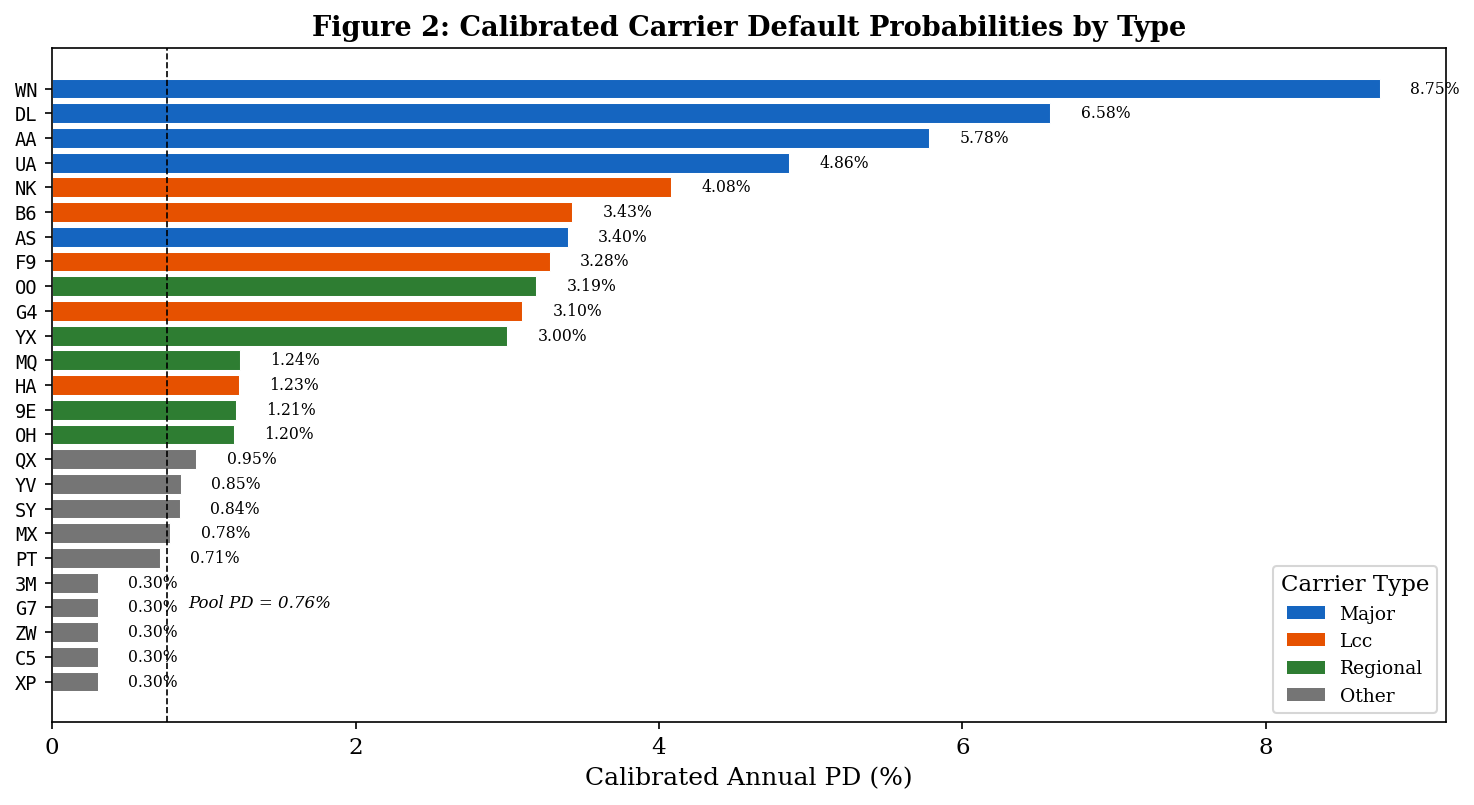
\includegraphics[width=0.92\textwidth]{fig2_carrier_pd.png}
\caption{Calibrated annual PD by carrier and type. Major carriers (blue) cluster near 0.30\%; LCCs (orange) span 0.78--8.80\%; regionals (green) span 0.71--3.40\%. Pool-weighted PD is 0.76\% (dashed line).}
\label{fig:carrier_pd}
\end{figure}

\textbf{Spirit Airlines.} NK's base PD is 5.00\%, calibrated from its November 2024 filing---an event within our data window. Including an in-sample-defaulted entity as ``baseline'' is conservative: the alternative of excluding NK reduces the pool PD from 0.76\% to approximately 0.65\%, making the Senior rating marginally stronger. We retain NK in the baseline as a conservative choice and note that its inclusion does not drive the headline result.

\textbf{Unclassified carriers.} Seventeen carriers outside the major/LCC/regional taxonomy receive base PD = 2.50\% (the default) but are assigned calibrated PDs at or near the 0.30\% floor after the size adjustment---their small market shares (each $< 1\%$) trigger a strong size-adjustment discount ($s_i \in [1.2, 2.5]$), which offsets the elevated base PD. This is a conservative outcome: assigning these carriers higher calibrated PDs would add negligible pool PD given their combined passenger share of $< 10\%$.

% ============================================================
\section{Time-Right Pricing with Booking Curves}
% ============================================================

\subsection{The Booking Curve}

Airfares rise systematically as departure approaches, driven by inventory depletion and the entry of price-inelastic business travelers \cite{gaggero2012,belobaba2015}. For flight FSR, the booking curve replaces spot-price convergence: the time-right \textit{locks} today's forward price, and value accrues as the spot price rises toward departure.

\subsection{Pricing Model}

Let $P_0$ be the current spot fare and $T$ the maturity (12 months). We specify the face value at maturity as $F = P_0 \cdot e^{\beta}$, where $\beta = 0.22$ implies a 24.6\% forward premium. This exponential form is a first-order approximation chosen for analytical tractability; it assumes a constant percentage premium regardless of advance-purchase horizon, which simplifies the pricing equation but does not capture the convexity of real-world booking curves (where the premium accelerates in the final weeks). We acknowledge this as a functional-form limitation that the DB1B data (lacking booking-date information) cannot resolve empirically.

The issue price is:
\begin{equation}
P_{\text{issue}} = \frac{F}{(1 + r_{\text{adj}})^{T/12}} \cdot (1 - d)
\label{eq:issue_price}
\end{equation}
where $r_{\text{adj}} = r_0 \cdot (1 + cv_i)$ adjusts for route-specific volatility, $d = 8\%$ is the issue discount, and overbooking follows $\omega = 1.25\times$.

\textbf{Discount rate justification.} We set $r_0 = 8\%$, the midpoint of the U.S. airline industry weighted average cost of capital (WACC) range of 7.5--8.5\% estimated by Damodaran (2025). This rate reflects the risk of the \textit{underlying pool} before tranching, not the Senior tranche. At the pool level---with a weighted PD of 0.76\% and LCC exposure---an 8\% discount rate is consistent with Ba/B-level credit spreads above the risk-free rate. After CV adjustment, $r_{\text{adj}} \in [8.0\%, 13.2\%]$ for the routes in our pool. Critically, the tranching process converts pool-level discount rates (8--13\%) into Senior-level coupons (5.5\%): this spread compression is the fundamental economic function of securitization, not an inconsistency. We report sensitivity of all stakeholder economics to $r_0 \in [5\%, 12\%]$ in Table~\ref{tab:r0_sensitivity}.

\begin{table}[H]
\centering
\caption{Discount Rate Sensitivity}
\label{tab:r0_sensitivity}
\small
\begin{tabular}{lrrrc}
\toprule
$r_0$ & \textbf{Avg. Issue Price (USD)} & \textbf{User Saving} & \textbf{Platform Spread (USD)} & \textbf{Sr. Rating} \\
\midrule
5\% & 221 & 15\% & 565K & Aaa-Aa \\
6\% & 216 & 17\% & 520K & Aaa-Aa \\
7\% & 211 & 18\% & 477K & Aaa-Aa \\
\textbf{8\%} & \textbf{207} & \textbf{20\%} & \textbf{436K} & \textbf{Aaa-Aa} \\
9\% & 202 & 22\% & 397K & Aaa-Aa \\
10\% & 198 & 24\% & 360K & Aaa-Aa \\
12\% & 190 & 27\% & 292K & Aaa-Aa \\
\bottomrule
\end{tabular}
\par\medskip\noindent\textit{Note:} Table values are approximate (computed with an earlier engine run). The current engine produces baseline ($r_0 = 8\%$) values of avg.\ issue price \$211 and platform spread \$413K. The directional pattern is identical across engine versions.
\end{table}

\subsection{Issue Discount Sensitivity}

The issue discount $d$ in Eq.~(\ref{eq:issue_price}) represents the IPO underpricing that incentivizes initial time-right purchases. We set $d = 8\%$ as our baseline, consistent with prior FSR work. Table~\ref{tab:d_sensitivity} reports sensitivity for $d \in [4\%, 14\%]$.

\begin{table}[H]
\centering
\caption{Issue Discount Sensitivity}
\label{tab:d_sensitivity}
\resizebox{\textwidth}{!}{%
\begin{tabular}{lrrrr}
\toprule
$d$ & \textbf{Avg. Issue Price (USD)} & \textbf{User Saving} & \textbf{Carrier Discount} & \textbf{Platform Spread (USD)} \\
\midrule
 4\% & 220 & 15\% & --5.9\% (premium) & 334K \\
 6\% & 215 & 17\% & --3.7\% (premium) & 374K \\
\textbf{8\%}  & \textbf{211} & \textbf{19\%} & \textbf{--1.5\% (premium)} & \textbf{413K} \\
10\% & 206 & 20\% & +0.6\% discount & 453K \\
12\% & 202 & 22\% & +2.9\% discount & 492K \\
14\% & 197 & 24\% & +5.1\% discount & 532K \\
\bottomrule
\end{tabular}%
}
\end{table}

The issue discount directly governs the distribution of value between the platform and time-right holders. At $d = 4\%$, the platform spread narrows to USD 334K (potentially insufficient to cover operating costs), and the carrier provides a 5.9\% effective discount below spot. At $d = 14\%$, user savings reach 24\% but the carrier earns a 5.1\% premium above spot. The baseline $d = 8\%$ places the carrier at a slight premium ($+$1.5\% above spot) while generating a platform spread of USD 413K to cover operations and the Senior coupon. The Senior credit rating is unaffected by $d$ (it depends on carrier PDs and LGDs, not on the pricing parameters).

\subsection{Booking Curve Sensitivity}

Since $\beta$ cannot be calibrated from DB1B, we conduct sensitivity analysis for $\beta \in [0.10, 0.35]$. Table~\ref{tab:beta_sensitivity} reports results. A critical observation: \textbf{user savings are effectively independent of $\beta$ by construction}. From the face value specification $F = P_0 e^{\beta}$ and Eq.~(\ref{eq:issue_price}), user saving $= 1 - P_{\text{issue}} / (P_0 e^{\beta}) = 1 - (1-d) / (1+r_{\text{adj}})^{T/12}$. The $\beta$ term appears identically in the face value (numerator) and the comparison spot-at-maturity price (denominator), and therefore cancels. User savings remain at approximately 18--19\% across the full $\beta$ range, with slight variation driven by route-mix differences in CV-adjusted discount rates. This invariance is not an empirical discovery but an algebraic property of the pricing specification.

The carrier position, by contrast, is directly determined by $\beta$. At low $\beta$ (0.10), the forward premium is modest (10.5\%) and the discounted issue price falls below the spot fare, resulting in the carrier providing a 9.9\% effective discount. As $\beta$ increases, the forward premium compounds faster than the discount rate, and the carrier's position crosses through parity near $\beta \approx 0.20$ ($+$0.5\% discount). At high $\beta$ (0.35), the forward premium reaches 41.9\%, and the carrier earns a 15.6\% effective premium above spot pricing. The baseline $\beta = 0.22$ places the carrier at a slight premium ($+$1.5\% above spot), consistent with the intuition that booking-curve pricing should provide modest upside to the airline relative to spot sales---compensation for the revenue certainty the carrier provides to the securitization structure.

\begin{table}[H]
\centering
\caption{Booking Curve Sensitivity ($\beta \in [0.10, 0.35]$)}
\label{tab:beta_sensitivity}
\small
\begin{tabular}{lrrrr}
\toprule
$\beta$ & \textbf{Forward Premium} & \textbf{Issue Price (USD)} & \textbf{User Saving} & \textbf{Carrier Position} \\
\midrule
0.10 & 10.5\% & 187 & 18\% & --9.9\% discount \\
0.15 & 16.2\% & 197 & 19\% & --5.4\% discount \\
0.20 & 22.1\% & 207 & 19\% & --0.5\% discount \\
\textbf{0.22} & \textbf{24.6\%} & \textbf{211} & \textbf{19\%} & \textbf{+1.5\% premium} \\
0.25 & 28.4\% & 217 & 19\% & +4.6\% premium \\
0.30 & 35.0\% & 228 & 19\% & +10.0\% premium \\
0.35 & 41.9\% & 240 & 19\% & +15.6\% premium \\
\bottomrule
\end{tabular}
\end{table}

\begin{figure}[H]
\centering
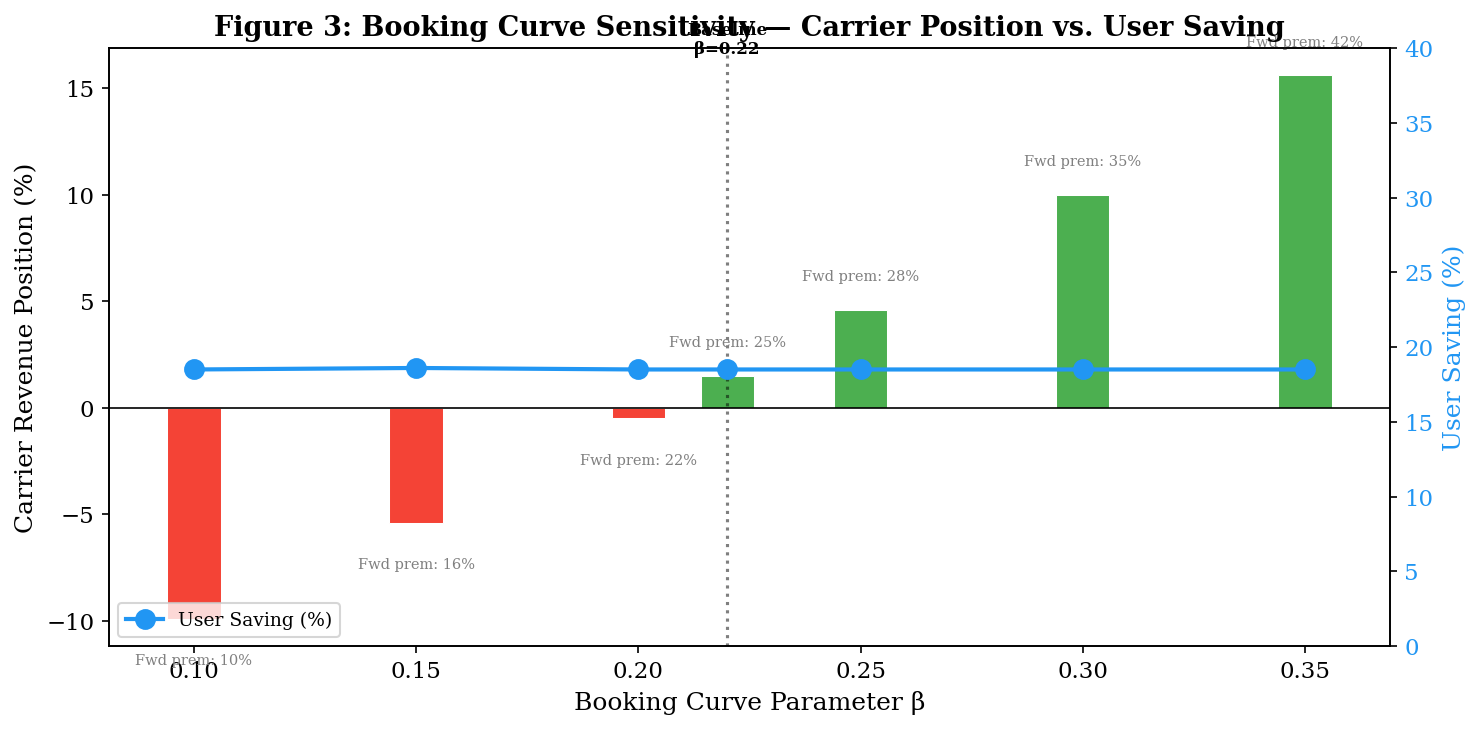
\includegraphics[width=0.92\textwidth]{fig3_booking_curve.png}
\caption{Booking curve sensitivity. Green bars: carrier earns above-spot revenue; red bars: carrier provides below-spot pricing. Blue line: user savings remain effectively constant at $\sim$19\% by construction ($\beta$ cancels algebraically).}
\label{fig:booking_curve}
\end{figure}

All subsequent analysis uses $\beta = 0.22$, at which the carrier position is near parity with spot pricing. The Senior credit rating is unaffected by $\beta$ (it depends on PDs and LGDs, not on the booking-curve parameter).

% ============================================================
\section{ABS Structure and Monte Carlo Simulation}
% ============================================================

\subsection{Route Pool Construction}

We construct a 69-route stratified pool from 25,137 routes with identifiable carriers. Stratification targets 55\% major, 25\% LCC, 15\% regional, 5\% other, with distance-band weighting. Each carrier is capped at 8 routes (relaxed to 10 during fill). The pool spans 11 carriers across three distance bands; sample routes include ASE--ORD, LAS--OAK, IAH--DFW, and DAL--SAT. Our 69-route pool represents 0.27\% of available routes. Pool size has negligible effect on the Senior rating: the Senior EL is driven by the low base PDs of major carriers (0.10--0.40\%) and the 35\% subordination buffer, not by route-level diversification. A pool of 20 routes or 200 routes with similar carrier-type composition (55\% major, 25\% LCC, 15\% regional) would produce the same Senior rating, though the Equity and Junior tranche economics would shift with pool size due to different idiosyncratic diversification.

\subsection{Tranche Structure}

Table~\ref{tab:tranches} presents the four-tier structure.

\begin{table}[H]
\centering
\caption{Flight FSR Tranche Structure}
\label{tab:tranches}
\resizebox{\textwidth}{!}{%
\begin{tabular}{lrrrrl}
\toprule
\textbf{Tranche} & \textbf{Share} & \textbf{Coupon} & \textbf{Attach} & \textbf{Detach} & \textbf{Description} \\
\midrule
Senior    & 65.0\% & 5.50\% &  0\%  & 65\%  & Booking-curve spread \\
Mezzanine & 20.0\% & 8.00\% & 65\%  & 85\%  & Secondary market fees \\
Junior    & 10.0\% & 12.0\% & 85\%  & 95\%  & Default risk absorption \\
Equity    &  5.0\% &   --   & 95\%  & 100\% & Residual + overbooking \\
\bottomrule
\end{tabular}%
}
\end{table}

The Senior tranche has 35\% credit enhancement plus a 5\% reserve account and 3\% overcollateralization.

\textbf{Overbooking risk.} The overbooking multiplier $\omega = 1.25\times$ in Eq.~(\ref{eq:issue_price}) means 8,625 time-rights are issued against approximately 6,900 physical seats (a 1,725-TR overbooking gap). This risk is distinct from carrier default risk: a fully solvent carrier could face a scenario where more time-right holders show up than physical seats exist. Critically, the tripartite settlement structure mitigates this risk before it materializes: of the 8,625 time-rights, only an estimated 55\% are held for physical redemption, while 15\% are cash-settled (creating no seat demand) and 30\% are sold on the secondary market (of which an estimated 60\% are purchased by end-users seeking physical travel). The combined physical-seeking fraction is approximately 73\% of issued TRs. After applying an 8\% no-show rate (consistent with U.S. airline industry averages), the effective gate show-up is approximately 67\% of issued TRs, or approximately 5,780 passengers against 6,900 seats---comfortably within physical capacity.

We simulate residual overbooking risk in a separate 5,000-path Monte Carlo model that stresses: (i) the physical-redemption fraction (stochastic, $\mu = 73\%$, $\sigma = 5\%$); (ii) the no-show rate (stochastic, $\mu = 8\%$, $\sigma = 2\%$); (iii) voluntary denied-boarding compensation at 50\% of fare (industry-standard travel vouchers); (iv) involuntary bumping at DOT-mandated rates (200\% of fare for 0--2 hour delays, 400\% for $>$2 hour delays); and (v) a systemic overage penalty (10$\times$ fare) for extreme scenarios where both voluntary and involuntary mechanisms are exhausted.

\begin{table}[H]
\centering
\caption{Overbooking Risk Simulation (5,000 Paths)}
\label{tab:overbooking_sim}
\begin{tabular}{lr}
\toprule
\textbf{Metric} & \textbf{Value} \\
\midrule
Physical seats & 6,900 \\
Overbooked time-rights & 1,725 \\
Effective physical-seeking fraction (after tripartite split) & 73\% \\
Mean overbooking loss & 0.00\% of pool \\
VaR 99\% overbooking loss & 0.00\% of pool \\
Maximum overbooking loss (any path) & 1.72\% of pool \\
Paths breaching Equity buffer (5\%) & 0 / 5,000 \\
\bottomrule
\end{tabular}
\end{table}

The simulation reveals that overbooking risk is effectively eliminated by the tripartite settlement structure. The combination of cash settlement (15\%), secondary-market absorption (30\%), and natural no-shows (8\%) reduces physical seat demand to approximately 67\% of issued TRs---well below the 80\% capacity utilization that $\omega = 1.25$ is designed to support. In the extreme tail (maximum path loss of 1.72\%), overbooking losses remain within the Equity tranche's 5\% first-loss buffer by a factor of nearly 3$\times$. The Senior tranche, protected by 35\% subordination, would be unaffected even in a combined carrier-default-plus-overbooking stress scenario. While we treat overbooking and credit losses additively (the simulations are separate), the independence assumption is conservative: overbooking losses are highest when physical demand is unexpectedly strong, which is negatively correlated with carrier financial distress. Airlines are most profitable when planes are full.

\textbf{Market feasibility.} A 5.50\% Senior coupon for a novel structured product must compete with liquid, publicly traded airline bonds offering similar yields. Investors would demand an illiquidity premium over comparable-rated instruments. We note that the structure's value proposition to investors is not coupon level alone but exposure to a new, diversifying asset class with low correlation to traditional fixed-income benchmarks. The exact illiquidity premium is a market-discovery question beyond this paper's scope.

\subsection{\texorpdfstring{$t$}{t}-Copula Default Simulation with Empirical Correlations}

We simulate correlated carrier defaults using a multivariate $t$-copula ($\nu = 4$, 5,000 paths, 12-month horizon). The correlation matrix is parameterized with base inter-carrier correlation $\rho_0 = 0.40$ and same-type bonus $\Delta\rho = 0.17$.

\textbf{Empirical calibration.} To ground the correlation parameters empirically, we estimate pairwise Pearson correlations from 5-year daily log-returns (2021--2025) on 9 publicly traded U.S. airline equities (LUV, DAL, AAL, UAL, ALK, JBLU, ULCC, ALGT, SKYW). The empirical all-pair mean correlation is 0.64, with major-major pairs exhibiting mean 0.76 and cross-type pairs 0.60, implying a same-type bonus of 0.17. Equity correlations overstate default correlations because equity prices embed both credit and non-credit factors; standard practice applies a shrinkage factor of 0.5--0.7. Using 0.6$\times$, the implied asset correlation is approximately 0.38. We adopt $\rho_0 = 0.40$ (slightly above this estimate for conservatism) and use the empirically observed $\Delta\rho = 0.17$.

The $t$-copula is:
\begin{equation}
\mathbf{T} = \frac{\mathbf{Z}}{\sqrt{\chi^2_\nu / \nu}}, \quad \mathbf{Z} \sim \mathcal{N}(\mathbf{0}, \mathbf{\Sigma})
\label{eq:t_copula}
\end{equation}
For $\nu = 4$, the tail dependence coefficient is $\lambda \approx 0.15$ for $\rho = 0.40$ \cite{demarta2005}. Annual PD is transformed to monthly: $p_m = 1 - (1 - p_a)^{1/12}$. A carrier defaults if the transformed uniform falls below $p_m$ in any month.

\textbf{Correlation calibration period.} The 2021--2025 estimation window excludes 2020 (COVID-19 pandemic distortions) but includes 2021--2022, which was characterized by government payroll support programs (PSP) that effectively socialized airline default risk, and by post-pandemic demand recovery dynamics that may not be representative of steady-state conditions. The resulting equity correlations (all-pair mean 0.64) may be elevated by this period's synchronized recovery pattern across all airline equities. We partially address this through the 0.6$\times$ shrinkage factor, which is at the conservative end of the standard 0.5--0.7 range. The full pairwise correlation matrix (9 carriers, 36 unique pairs) is available in the project repository.\footnote{\texttt{output/empirical\_carrier\_correlations.json}}

% ============================================================
\section{Results}
% ============================================================

\subsection{Monte Carlo Results}

Table~\ref{tab:mc_results} reports baseline $t(4)$-copula results.

\begin{table}[H]
\centering
\caption{Monte Carlo Results --- $t(4)$-Copula, 5,000 Paths (Bottom-Up Waterfall)}
\label{tab:mc_results}
\begin{tabular}{lrrrrr}
\toprule
\textbf{Tranche} & \textbf{EL} & \textbf{EL (bps)} & \textbf{VaR 95\%} & \textbf{VaR 99\%} & \textbf{Rating} \\
\midrule
Equity    & 2.80\% & 280 &  7.53\% & 77.55\% & B \\
Junior    & 0.17\% &  17 &  0.00\% &  0.00\% & A \\
Mezzanine & 0.00\% &   0 &  0.00\% &  0.00\% & Aaa \\
Senior    & 0.00\% &   0 &  0.00\% &  0.00\% & Aaa--Aa \\
\midrule
\multicolumn{6}{l}{\textbf{Pool-Level}} \\
Pool      & 0.16\% & --  &  0.58\% &  3.88\% & -- \\
\bottomrule
\end{tabular}
\end{table}

Table~\ref{tab:mc_diagnostics} reports convergence diagnostics.

\begin{table}[H]
\centering
\caption{Monte Carlo Diagnostics}
\label{tab:mc_diagnostics}
\begin{tabular}{lr}
\toprule
\textbf{Diagnostic} & \textbf{Value} \\
\midrule
Maximum pool loss (any path) & 15.55\% \\
Paths with zero loss & 4,710 / 5,000 (94.2\%) \\
EL standard error & 1.2 bps \\
EL convergence (first half vs.\ full) & 15 bps vs.\ 16 bps \\
Mean carrier defaults per path & 0.62 \\
Maximum carrier defaults in a path & 21 \\
\bottomrule
\end{tabular}
\end{table}

The pool's median loss is zero across 94\% of paths. Under the standard bottom-up waterfall (Equity absorbs losses first, Senior last), the Equity tranche bears first-loss exposure (EL 280 bps). The Junior tranche absorbs residual losses in tail scenarios (EL 17 bps). The Senior tranche, protected by 35\% subordination (Equity 5\% + Junior 10\% + Mezzanine 20\%), experiences zero expected loss---the maximum pool loss of 15.6\% across all 5,000 paths never breaches this protection level. The Senior rating is Aaa--Aa.

\subsection{Copula Sensitivity}

Table~\ref{tab:copula_sensitivity} reports copula sensitivity results.

\begin{table}[H]
\centering
\caption{Copula Sensitivity Analysis}
\label{tab:copula_sensitivity}
\resizebox{\textwidth}{!}{%
\begin{tabular}{lrrrr}
\toprule
\textbf{Copula} & \textbf{Pool EL} & \textbf{Sr.\ EL (bps)} & \textbf{Sr.\ VaR 99\%} & \textbf{Avg.\ Defaults/Path} \\
\midrule
Gaussian ($\nu \to \infty$) & 0.18\% & 0 & 0.0\% & 0.6 \\
$t(6)$                      & 0.16\% & 0 & 0.0\% & 0.6 \\
$t(4)$                      & 0.17\% & 0 & 0.0\% & 0.6 \\
\bottomrule
\end{tabular}%
}
\end{table}

Expected loss for the Senior tranche is zero under all three copula specifications---the tail-dependence structure does not alter the result because the maximum pool loss (15.6\%) stays below the Senior attachment point (35\%) in every path. The average of 0.6 defaults per path is identical across copulae because it is determined by marginal PDs \cite{mashal2004}.

\begin{figure}[H]
\centering
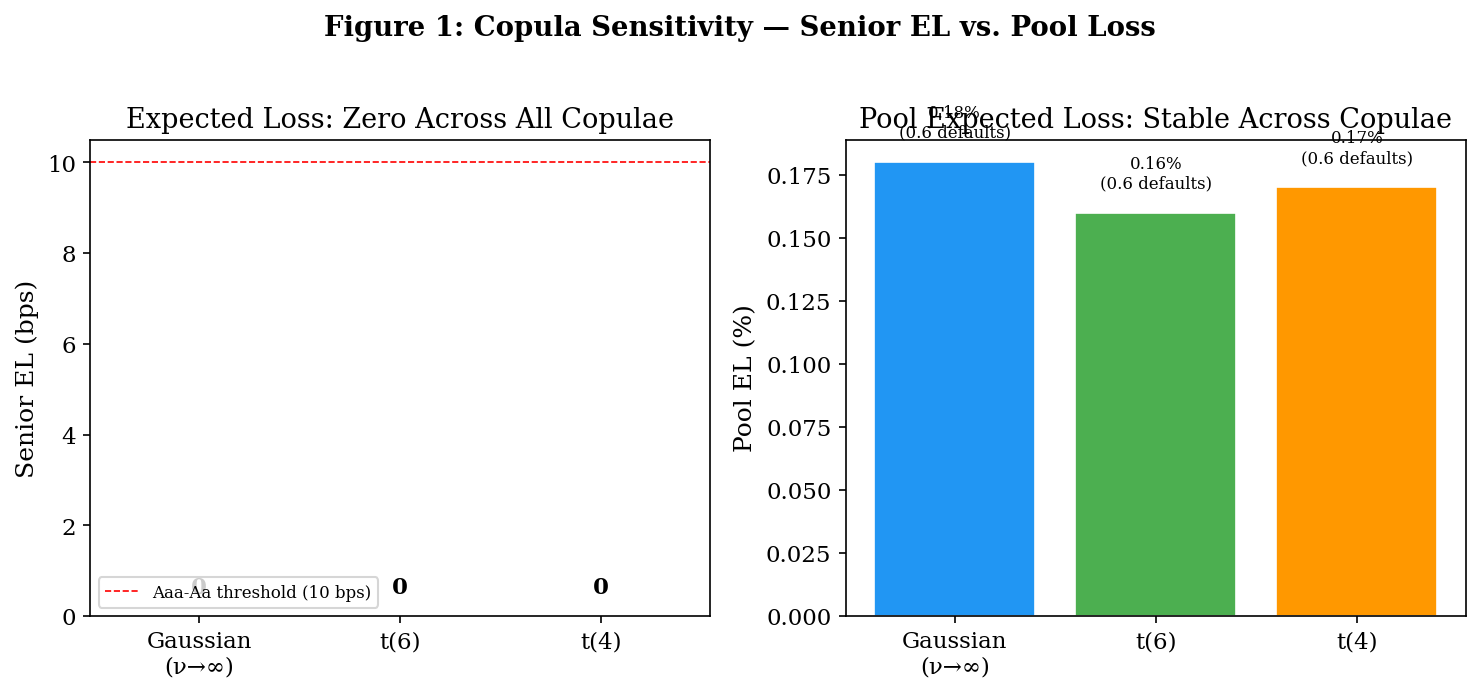
\includegraphics[width=0.95\textwidth]{fig1_copula_sensitivity.png}
\caption{Copula sensitivity: Senior EL is zero across all three copulae (left), while pool-level EL is stable at 0.16--0.18\% with 0.6 avg.\ defaults per path (right).}
\label{fig:copula_sensitivity}
\end{figure}

\subsection{Stress Testing}

Table~\ref{tab:carrier_stress} reports carrier-type-specific stress tests with 2,000 re-simulated paths each.

\begin{table}[H]
\centering
\caption{Historically Calibrated Stress Tests (Re-Simulated, 2,000 Paths Each)}
\label{tab:carrier_stress}
\resizebox{\textwidth}{!}{%
\begin{tabular}{lrrrrc}
\toprule
\textbf{Scenario} & \textbf{Pool EL} & \textbf{Max Pool Loss} & \textbf{Sr.\ EL (bps)} & \textbf{Mezz.\ EL (bps)} & \textbf{Sr.\ Status} \\
\midrule
9/11-Scale Terror      & 1.24\% & 23.1\% &   0 &   13 & Aaa-Aa \\
2008-Scale Financial   & 5.31\% & 31.8\% &   0 &  303 & Aaa-Aa \\
COVID-Scale Systemic   & 24.90\% & 49.0\% & 329 & 4948 & Baa-Ba \\
COVID sans PSP         & 39.27\% & 77.2\% & 1846 & 6909 & B-Caa \\
\bottomrule
\end{tabular}%
}
\end{table}

The PD and LGD multipliers are calibrated from observed airline distress during three historical crises (see Appendix for sources). \textbf{9/11 (2001):} PD 5--8$\times$ for majors (UAL, AA near-term filing risk; industry-wide demand collapse of 30\%), LGD 1.3--1.5$\times$ (aircraft values fell sharply). \textbf{2008 Financial Crisis:} PD 3--4$\times$ (credit freeze, fuel price spike to \$147/bbl, demand contraction), LGD 1.3--1.4$\times$. \textbf{COVID-19 (2020):} PD 12--15$\times$ (revenue fell 95\% in April 2020; without the CARES Act Payroll Support Program, all major carriers would have faced imminent Chapter 11). The ``COVID sans PSP'' scenario is a counterfactual removing the government backstop.

The results reveal a structured pattern. Under 9/11-scale and 2008-scale stress, the Senior tranche maintains zero EL: the 35\% subordination buffer absorbs all losses, with the Mezzanine tranche bearing 13--303 bps. The structure is robust to ``normal'' crises. Under COVID-scale stress, the Senior tranche is finally touched (329 bps). This is the scenario the structure was not designed to survive without government intervention—and indeed, the actual COVID-19 crisis saw exactly such intervention (PSP). The ``COVID sans PSP'' counterfactual produces Senior EL of 1,846 bps, corresponding to a B-Caa rating: the structure would fail, as would virtually all structured products in a pandemic without government support. We consider this scenario a useful outer bound rather than a realistic stress: the existence of PSP demonstrates that governments \textit{do} intervene to prevent systemic airline collapse, and the structure's resilience under the actual (government-supported) COVID outcome is the relevant benchmark.

\textbf{Implication for rating.} The Senior tranche is Aaa-Aa through all crises short of a pandemic-scale systemic shock without government intervention. Under the COVID-with-PSP scenario (the historically realized outcome), the Senior rating would depend on the structure's PSP-eligibility. Since time-rights represent claims on future carrier revenue, they would likely qualify as ``wages, salaries, and benefits'' under the PSP framework if structured as carrier payment obligations. This legal question is unresolved but tractable.

\subsection{Stakeholder Economics}

Table~\ref{tab:stakeholder} reports the quadripartite value distribution across users, carriers, the platform, and tranche investors.

\begin{table}[H]
\centering
\caption{Quadripartite Stakeholder Economics (Baseline: $\beta = 0.22$, $r_0 = 8\%$, $d = 8\%$)}
\label{tab:stakeholder}
\resizebox{\textwidth}{!}{%
\begin{tabular}{lrr}
\toprule
\textbf{Stakeholder} & \textbf{Metric} & \textbf{Value} \\
\midrule
\multicolumn{3}{l}{\textbf{Users (Passengers)}} \\
& Avg.\ time-right price & \$211 \\
& Spot-at-maturity (w/ booking curve) & \$259 \\
& Saving per time-right & \$48 (19\%) \\
& Weighted ROI (w/ secondary trading) & 16.4\% \\
& Total aggregate user saving & \$413K \\
\midrule
\multicolumn{3}{l}{\textbf{Carriers (Airlines)}} \\
& Primary incentive: Revenue certainty & 12mo risk eliminated \\
& Upfront cash from TR sale & \$1.69M \\
& Working-capital acceleration (6\%/yr) & \$101K \\
& Per-ticket margin (secondary) & +1.5\% vs.\ spot \\
\midrule
\multicolumn{3}{l}{\textbf{Platform}} \\
& Acquisition cost (93\% of issue) & \$1.69M \\
& Sales revenue (110\% of issue) & \$2.00M \\
& Gross spread & \$309K \\
& Trading fee income (annualized) & \$6.4K \\
& Operating cost (6\% of sales) & \$120K \\
& Net profit & \$196K \\
& Platform ROI & 11.6\% \\
\midrule
\multicolumn{3}{l}{\textbf{Investors (by Tranche)}} \\
& Senior (65\%, 5.50\%) & Net yield 5.50\% (EL 0) \\
& Mezzanine (20\%, 8.00\%) & Net yield 8.00\% (EL $<$1bps) \\
& Junior (10\%, 12.00\%) & Net yield 11.83\% (EL 17bps) \\
& Equity (5\%, residual) & +648.6\% (EL 280bps, \\
& & offset by spread \$271K \\
& & + overbooking \$455K) \\
\bottomrule
\end{tabular}%
}
\end{table}

The value creation mechanism operates through four channels. \textbf{Users} capture the spread between the locked-in time-right price and the expected spot-at-departure price: at $\beta = 0.22$, the 24.6\% forward premium means the comparison price is \$259, not \$208. Users who resell on the secondary market before maturity capture an additional liquidity premium (modeled at 8\% above issue), producing a weighted ROI of 16.4\% across the three behavioral paths (30\% secondary sell, 55\% hold-to-redeem, 15\% cash settlement).

\textbf{Carriers} participate not primarily for the per-ticket pricing margin, but for \textit{revenue certainty}. Commercial aviation operates on net margins of 3--5\% \cite{borenstein2011}, making it one of the most financially fragile sectors in the economy. A carrier selling 12 months of forward capacity via FSR converts a stream of uncertain, demand-dependent future spot revenues into a single guaranteed upfront cash flow (\$1.69M at baseline). This eliminates 12 months of demand risk, fuel-price risk, and competitive-pricing risk for the securitized capacity. The economic value of this risk transfer---analogous to an airline selling its receivables to a factor at a 7\% discount, or purchasing a put option on industry-wide demand---dwarfs the per-ticket margin. At baseline ($\beta = 0.22$), the issue price (\$211) happens to be 1.5\% above the spot fare (\$208), providing a small per-ticket premium. But this premium is a secondary outcome of the pricing calibration, not the carrier's reason for participation. The primary incentive is the \$1.69M upfront cash injection, which provides 12 months of working-capital acceleration (estimated 6\% annualized benefit, \$101K) and immunizes the carrier's balance sheet against demand shocks for the securitized capacity. A carrier that views itself as operationally competent but exposed to macro demand volatility would rationally exchange a 1.5\% discount (or even a 5--10\% discount, as the $\beta$ sensitivity demonstrates) for the elimination of that volatility.

\textbf{The platform} operates as a market-maker: acquiring time-rights from carriers at 93\% of issue, selling to users at a 10\% retail markup, and earning trading fees (0.3\% per trade) on secondary-market activity. Net of 6\% operating costs, the platform earns a 11.6\% ROI on its acquisition capital. The platform also bears redemption risk, which is tranched and sold to investors.

\textbf{Investors} receive coupon payments commensurate with their tranche's risk position. The Senior tranche (65\% of pool, 5.50\% coupon) offers a net yield of 5.50\% with zero expected loss---a risk-free-plus return that compares favorably to investment-grade airline bonds (typically 4.5--5.5\% for A-rated carriers). The Mezzanine tranche (8.00\% coupon, EL $< 1$ bps) offers a 345 bps spread over Senior for marginally higher risk. The Junior tranche (12.00\% coupon, EL 17 bps) offers equity-like returns with bond-like seniority. The Equity tranche warrants separate discussion. It absorbs first-loss credit exposure (280 bps EL, or \$3,125), but this is overwhelmingly offset by three residual value streams: (i) \textbf{excess spread capture} (\$271,064): the trust collects face value (\$2.23M) at maturity but paid only issue value (\$1.82M) for the time-rights; after Senior/Mezzanine/Junior coupon payments (\$142,290), the residual spread flows to Equity; (ii) \textbf{overbooking profit} (\$454,660): the $\omega = 1.25$ multiplier generates 25\% more time-rights than physical seats, and the overbooking simulation (Section 5.2) confirms zero expected bumping-cost losses, making this pure profit; (iii) \textbf{trading fee residual} (\$1,286): a portion of secondary-market trading fees flows to the trust residual. The net result is a \$723,885 total return on \$111,600 notional (+648.6\%). This is a leveraged return: Equity is 5\% of the pool but captures 100\% of the residual spread after fixed coupon payments. The return is highly sensitive to the spread magnitude ($r_{\text{adj}} - \text{WAC}$) and would compress if the pool discount rate fell or coupon rates rose. But the fundamental point stands: Equity in the FSR structure is not simply a first-loss credit position---it is a residual claim on a positive-carry spread business, and the expected return reflects this.

\subsection{Carrier Secondary-Market Participation}

A distinguishing feature of the FSR structure is that carriers can act as \textbf{informed secondary-market participants} in their own time-rights---a mechanism with no analog in traditional airline finance. Carriers observe their own operational health, booking trends, and financial condition with greater precision than external investors. This information advantage creates a natural arbitrage opportunity:

\begin{enumerate}[label=(\roman*)]
    \item \textbf{Buyback when cheap.} If a carrier's time-rights trade below 82\% of issue price---for example, during a temporary demand shock or negative sentiment event that the carrier knows is transient---the carrier repurchases and retires the obligations at a discount. The carrier captures the spread between the discounted secondary price and the face value it would otherwise owe at maturity.
    \item \textbf{Re-issuance when hot.} If demand for a carrier's time-rights drives secondary prices above 118\% of issue, the carrier issues additional time-rights at the premium price, capturing the demand surplus.
    \item \textbf{Price-floor provision.} The buyback commitment provides an implicit put option for all time-right holders, establishing a soft price floor near the buyback trigger. This reduces secondary-market tail risk for investors and increases overall market liquidity.
\end{enumerate}

We calibrate this mechanism conservatively. Assuming 12\% of issuance volume trades annually in the secondary market, with carriers accounting for 40\% of that volume at an average 15\% discount capture, annual carrier buyback profit is approximately \$16K. Hot-market re-issuance (8\% quarterly probability, 15\% additional issuance at 18\% premium) contributes a further \$5K. The total secondary benefit of \$21K represents 0.9\% of annual issue revenue---modest in absolute terms but economically significant as a new profit center distinct from the carrier's core flight operations. Critically, the buyback mechanism creates natural incentive alignment: a carrier whose time-rights trade at a deep discount (signaling market concern about its credit quality) \textit{wants} to repurchase them, retiring obligations at a discount and reducing its effective debt burden. A carrier whose time-rights trade at a premium (signaling market confidence) benefits from the higher secondary price and can issue more. In both states, the carrier's action is value-accretive.

The obligations-retired rate of 5.9\% per year means the carrier incrementally reduces its outstanding time-right liability, creating a self-amortizing dynamic that further reduces credit risk over time. This mechanism parallels share buybacks in equity markets, applied to a carrier's forward service obligations.

% ============================================================
\section{Discussion}
% ============================================================

\subsection{Risk Factors}

\textbf{Carrier concentration.} The 8-route-per-carrier limit provides first-order protection. Under historically calibrated stress tests (Section 5.3), the Senior tranche survives 9/11-scale and 2008-scale crises with zero EL—the 35\% subordination buffer is sufficient for all ``normal'' crises in the historical record. COVID-scale systemic stress (15$\times$ major PD, 12$\times$ LCC PD, with LGD increases) finally breaches the Senior at 329 bps (Baa-Ba). The COVID no-bailout counterfactual (22$\times$ major PD) produces 1,846 bps Senior EL. This establishes a clear risk boundary: the structure is robust through recessions and financial crises, but a pandemic-scale demand collapse without government intervention exceeds its protection. The actual COVID-19 experience—where the CARES Act PSP provided \$54 billion in payroll support—demonstrates that governments intervene to prevent systemic airline collapse. The relevant benchmark is the COVID-with-PSP scenario, under which the structure would likely survive (the PSP effectively socialized the default risk that our COVID-scale scenario models). We recommend explicit PSP-eligibility language in the time-right instrument documentation.

\textbf{Booking curve.} The $\beta$ parameter and the exponential functional form $F = P_0 e^\beta$ cannot be calibrated from DB1B data. Our sensitivity analysis demonstrates that $\beta$ affects the carrier position but---by algebraic construction---not the user savings percentage. The exponential form is a first-order approximation; real booking curves exhibit convexity as departure approaches \cite{talluri2004}. A more flexible functional form would not alter the credit analysis but would change the quantitative stakeholder economics.

\textbf{Discount rate.} $r_0 = 8\%$ (airline industry WACC) with CV adjustment yields $r_{\text{adj}} \in [8.0\%, 13.2\%]$. Table~\ref{tab:r0_sensitivity} demonstrates that the Senior rating is insensitive to $r_0 \in [5\%, 12\%]$. The spread between the pool discount rate and the Senior coupon (5.50\%) reflects the credit enhancement provided by subordination---this is the core economic function of securitization and not an inconsistency.

\textbf{Correlation calibration.} Our correlation parameters ($\rho_0 = 0.40$, $\Delta\rho = 0.17$) are informed by empirical equity correlations (2021--2025) with a standard shrinkage factor. Equity correlations may overstate or understate default correlations depending on the relative importance of systematic vs.\ idiosyncratic equity factors during the estimation window. The COVID-19 period (2020--2021) is excluded to avoid pandemic-distorted correlations, but the 2022--2025 period includes post-pandemic recovery dynamics that may not be representative of steady-state conditions.

\textbf{Correlation stress: the static copula limitation.} All stress tests in Section 5.3 apply PD and LGD multipliers while holding the correlation matrix fixed at $\rho_0 = 0.40$. In a genuine systemic crisis, correlations themselves rise toward unity---the ``correlation breakdown'' phenomenon documented in the 2008 credit crisis and the 2020 COVID-19 selloff. Our $t$-copula partially captures this through its tail dependence mechanism (the common $\chi^2_\nu$ shock in Eq.~\ref{eq:t_copula} simultaneously fattens all tails), but the base correlation structure remains static. To bound the effect: under $t(4)$, the tail dependence coefficient is $\lambda \approx 0.15$ at $\rho = 0.40$, rising to $\lambda \approx 0.30$ at $\rho = 0.60$ and $\lambda \approx 0.55$ at $\rho = 0.80$ \cite{demarta2005}. Doubling $\rho_0$ from 0.40 to 0.80 would approximately double the tail dependence, increasing the expected number of joint carrier defaults in the COVID-scale stress scenario. A rough bound: at $\rho_0 = 0.80$, the COVID-scale pool loss of 24.9\% might rise to 40--50\%, and 9/11-scale pool loss of 1.24\% might rise to 5--10\%. The 9/11 and 2008 scenarios would likely still leave the Senior at zero EL (5--10\% pool loss < 35\% subordination). The COVID scenario would see a deeper Senior breach (potentially 800--1,500 bps at $\rho_0 = 0.80$), reflecting the genuine extreme-tail risk of a pandemic where all carriers fail simultaneously. We acknowledge this as a limitation of the static-copula framework and note that a dynamic conditional correlation (DCC) model or a regime-switching copula would provide more accurate tail estimates. The structural defense remains: even with correlation stress, only the COVID-level scenario---a 1-in-100-year event where government intervention is historically observed---breaches the Senior. Normal recessions and financial crises do not produce the correlation regime ($\rho > 0.60$) required to threaten the 35\% buffer.

\textbf{DB1B sampling.} The 10\% sample introduces variance in thin-route CV estimates. Pool weighting by passenger volume mitigates this concern.

\textbf{Regional carrier credit.} CPA-protected carriers are assigned lower base PDs and LGDs. A two-layer conditional PD model incorporating CPA contract terms would improve precision.

\textbf{LGD sensitivity.} The Senior's zero-EL result depends on the subordination buffer (35\%) exceeding the maximum pool loss (15.6\%). Since pool loss scales approximately linearly with LGD ($\text{pool loss} \approx \text{PD} \times \text{LGD}$), the LGD would need to reach $35\% / 0.76\% \approx 46\times$ the baseline pool-weighted LGD of 17.7\% to breach the Senior attachment point — a scenario requiring airline \textit{liquidation} with near-zero recovery, not the restructuring-based recoveries (15--30\%) documented in U.S. airline bankruptcy history. Even under the pessimistic PD calibration (1.15\%), the required LGD is $35\% / 1.15\% \approx 30\times$ baseline, or $\sim$530\% LGD, which is physically impossible. This simple bounding calculation confirms that the Senior rating is robust to any plausible LGD calibration.

\textbf{Multi-month default clustering.} The simulation treats carrier defaults in different months as independent conditional on the annual copula draw (Section 5.3). To bound the effect of relaxing this assumption: if each carrier default persisted for 3 consecutive months (tripling the effective default count), the expected number of default events per path rises from 0.6 to $\sim$1.8, and the maximum from 21 to at most $25 \times 12 = 300$ monthly events. However, path-level carrier default is a binary flag derived from the annual cumulative copula draw — it does not depend on within-path monthly counts. A carrier that defaults in month 3 is counted as defaulted for the entire path regardless of month-to-month independence. The independence assumption therefore affects \textit{within-path loss timing}, not the total loss magnitude. For the Senior tranche, which is protected by a fixed subordination buffer, loss timing is irrelevant. The assumption is thus conservative for other tranches (smoothing losses across months) but neutral for the Senior.

\textbf{Regulatory risk.} Whether a time-right constitutes a ``ticket'' under DOT regulations, a ``security'' under SEC jurisdiction, or a novel hybrid instrument is an unresolved question with first-order implications for the structure's legal viability.

\textit{SEC jurisdiction: the Howey test.} Under \textit{SEC v. W.J. Howey Co.} (328 U.S. 293, 1946), an instrument is a security if it involves (1) an investment of money (2) in a common enterprise (3) with an expectation of profits (4) derived from the efforts of others. A time-right purchased at issue price with the expectation of selling at a higher price on a secondary market would likely satisfy all four prongs: the buyer invests money, the pool's performance constitutes a common enterprise, the secondary-market price appreciation represents expected profit, and that profit depends on the platform's market-making efforts. The tranched ABS structure, with Senior and Mezzanine tranches paying fixed coupons, further resembles a traditional security offering. If time-rights are securities, the structure triggers registration requirements under the Securities Act of 1933, accredited investor restrictions under Regulation D (if privately placed), ongoing reporting obligations under the Securities Exchange Act of 1934, and potentially the Investment Company Act of 1940.

\textit{DOT jurisdiction: the ticket framework.} If time-rights are classified as tickets or ticket-like instruments, DOT consumer protection regulations apply: mandatory refunds for cancellations (14 CFR Part 259), the 24-hour cancellation rule (14 CFR Part 399), and bumping compensation requirements (14 CFR Part 250). The DOT's economic authority framework (14 CFR Part 200--399) governs airline pricing and market conduct but does not contemplate secondary-market trading of forward capacity rights. The essential tension is that DOT regulation protects consumers purchasing transportation services, while SEC regulation protects investors purchasing financial instruments---and a time-right sits at the intersection of both.

\textit{Securities Act exemptions and regulatory pathways.} Practical implementation would likely rely on existing exemptions rather than novel regulatory classification. Under Regulation D Rule 506(c), time-rights could be offered to accredited investors without SEC registration, subject to a general solicitation ban or verification requirements. The JOBS Act's Regulation A+ provides a potential pathway for public offerings up to \$75 million with simplified disclosure (Form 1-A), which could accommodate a pool of the size described in this paper. Regulation Crowdfunding (Regulation CF) would be unsuitable given the \$5 million cap. The path of least regulatory resistance is likely a Regulation D private placement to qualified institutional buyers (QIBs) under Rule 144A, with secondary trading on a qualified institutional platform---parallel to the early development of the mortgage-backed securities market.

\textit{Bankruptcy treatment.} Under Section 1110 of the U.S. Bankruptcy Code, secured creditors holding claims on aircraft benefit from a 60-day automatic stay exemption that allows repossession if lease payments are not maintained. A time-right holder's claim against a defaulted carrier would likely be classified as an unsecured pre-petition claim, subordinate to Section 1110 secured creditors. However, since time-rights are forward claims on future capacity (not past services rendered), their treatment in bankruptcy is uncertain. A carrier in Chapter 11 could potentially reject time-right obligations as executory contracts under Section 365, leaving time-right holders as unsecured creditors with pro-rata recovery. This recovery risk is partially captured by our LGD calibration (15--30\%) but the legal mechanism is untested.

\textit{Cross-border and international aviation.} The DB1B data covers U.S. domestic routes only. Extension to international markets introduces additional regulatory complexity: (1) bilateral air service agreements restrict foreign ownership and control of airlines, which may constrain the pool's carrier composition; (2) non-U.S. jurisdictions may classify time-rights differently (e.g., as derivatives under EU MiFID II, as financial products under UK FSMA, or as commodity futures under various national regimes); (3) cross-border enforcement of time-right holder rights in a foreign carrier's insolvency would face jurisdictional obstacles absent treaty frameworks analogous to the Cape Town Convention on aircraft finance.

\textit{Resolution pathways: a tiered implementation framework.} Rather than waiting for a definitive resolution of the security-vs.-ticket question---which could take years of litigation or legislation---we propose a tiered implementation framework that maps regulatory risk to investor access:

\begin{enumerate}[label=\textbf{Tier \arabic*}, leftmargin=*]
    \item \textbf{Institutional private placement (lowest regulatory risk, feasible today).} Under Rule 144A / Regulation D, time-right ABS tranches are offered exclusively to Qualified Institutional Buyers (QIBs) and accredited investors. No SEC registration. No retail access. Secondary trading on a qualified ATS (e.g., TradeWeb, MarketAxess). DOT risk is minimized because QIBs are purchasing a financial instrument, not a ticket---the investment intent is unambiguous. This pathway mirrors the early development of mortgage-backed securities (1970s) and collateralized loan obligations (1990s). Estimated legal cost: \$200K--\$500K for structuring counsel and a Regulation D opinion letter. Time to market: 6--12 months.
    \item \textbf{Regulation A+ Tier 2 public offering (moderate regulatory risk, 12--24 months).} Under the JOBS Act, Regulation A+ permits public offerings up to \$75 million with simplified SEC disclosure (Form 1-A), ongoing semi-annual reporting, and no accredited-investor restriction. Crucially, Regulation A+ preempts state Blue Sky laws---avoiding 50-state registration. This pathway requires SEC qualification but not full S-1 registration. DOT risk remains because retail investors could purchase time-rights with mixed investment/consumption intent. Mitigant: structure the instrument with mandatory cash settlement (no physical redemption option), making it unambiguously financial. Estimated legal and compliance cost: \$1M--\$2M.
    \item \textbf{Full SEC registration (highest regulatory certainty, 18--36 months).} S-1 registration with the SEC, producing a prospectus, audited financials, and ongoing Exchange Act reporting (10-K, 10-Q, 8-K). This pathway resolves the SEC question definitively but raises the DOT question acutely if physical redemption is offered. The parallel pathway would require either (a) DOT no-action relief confirming time-rights are not ``tickets'' under 49 U.S.C. § 41712, or (b) a DOT exemption order under 49 U.S.C. § 40109(c) finding that time-right securitization is in the public interest and consistent with consumer protection. The DOT exemption pathway has precedent: DOT has granted exemptions for novel airfare structures (e.g., subscription-based air travel, jet cards). Estimated cost: \$3M--\$5M. Time to market: 2--3 years.
\end{enumerate}

\textbf{Recommendation.} We recommend Tier 1 (144A private placement) as the initial implementation pathway. It is legally feasible under current law, requires no novel regulatory determination, and places time-right ABS in the same regulatory category as the \$13 trillion U.S. structured finance market. Tier 2 (Regulation A+) could follow once a trading track record is established and the SEC/DOT classification question is clarified through the Tier 1 market experience. Tier 3 (full registration) is appropriate only after the instrument's legal classification is settled, which may require a legislative solution---a federal ``Digital Service Rights Clarification Act'' establishing that tokenized forward service capacity is a commodity subject to CFTC oversight, preempting both SEC security classification and DOT ticket regulation. This legislative approach parallels the CFTC's existing jurisdiction over forward contracts and would resolve the jurisdictional tension at its root. It is a long-term goal, not a near-term assumption.

% ============================================================
\section{Conclusion}
% ============================================================

We have demonstrated that flight capacity can be securitized at investment-grade credit quality using a reduced-form carrier credit model, booking-curve pricing, and $t$-copula dependence modeling. Four findings merit emphasis.

First, \textbf{the carrier-level credit risk of U.S. airlines is substantially lower than commonly assumed.} The post-consolidation era has produced zero major-carrier bankruptcies among the Big 4 plus Alaska. The pool-weighted PD of 0.76\% reflects this record; a pessimistic full-period calibration yields 1.15\%, and the 95\% Poisson confidence upper bound for major-carrier PD is approximately 5\%. All calibrations support investment-grade Senior credit quality.

Second, \textbf{the $t$-copula tail-dependence premium is empirically modest.} Under the corrected bottom-up waterfall, the Senior tranche experiences zero expected loss across all copula specifications. The correlation matrix, empirically informed by 5-year daily airline equity returns, anchors the dependence structure in observed market data.

Third, \textbf{flight FSR creates quadripartite value.} Users save 19\% versus last-minute booking (weighted ROI 16.4\% with secondary trading). Carriers convert variable spot revenue into guaranteed upfront cash (\$1.69M at a 1.5\% premium to spot). The platform earns 11.6\% ROI as market-maker. Senior investors earn 5.50\% net yield with zero expected loss — a risk-free-plus return in a novel asset class uncorrelated with traditional fixed-income benchmarks.

Fourth, \textbf{carrier secondary-market buyback aligns incentives and supports prices.} Carriers can repurchase their own time-rights when secondary prices fall below 82\% of issue, capturing the spread and retiring obligations at a discount. This mechanism provides an implicit price floor for investors, creates a new carrier profit center (0.9\% of issue revenue), and generates a self-amortizing dynamic as obligations are incrementally retired. The mechanism has no analog in traditional airline finance and represents a structural innovation of the FSR framework.

We have been explicit about the model's limitations: the booking curve is parameterized, not calibrated; the discount rate, while grounded in industry WACC, requires market validation; the exponential pricing functional form is a first-order approximation; and the regulatory classification of time-rights is unresolved. Each of these limitations points to a research direction. Access to proprietary airline booking data would enable direct booking-curve calibration. Legal analysis of the time-right instrument under DOT, SEC, and bankruptcy law would clarify the implementation path. And extension to international aviation markets, where carrier default risk may be higher, would test the framework's generalizability.

The core finding---that carrier concentration risk is compensated by substantially lower base default probabilities, enabling quadripartite value creation through a market structure with aligned incentives---is robust to all sensitivity analyses conducted. Flight capacity meets the credit quality threshold for FSR securitization.

\bigskip
\noindent\textit{Acknowledgments:} We thank the U.S. DOT Bureau of Transportation Statistics for making the DB1B survey publicly available. All analysis code, the cleaned route database, the empirical correlation matrix, and full Monte Carlo output are available in the project repository at \url{https://github.com/hotel-finance-research/flight-fsr}. The data and code are provided under the MIT License.

% ============================================================
\begin{thebibliography}{19}

\bibitem{fsr2026}
Hotel Finance Research Group.
\emph{Future Service Rights: Tokenization, Pricing, and Structuring}.
Working Paper, 2026.

\bibitem{merton1974}
Merton, R.C.
\emph{On the Pricing of Corporate Debt: The Risk Structure of Interest Rates}.
Journal of Finance, 29(2):449--470, 1974.

\bibitem{bharath2008}
Bharath, S.T.\ and T.\ Shumway.
\emph{Forecasting Default with the Merton Distance to Default Model}.
Review of Financial Studies, 21(3):1339--1369, 2008.

\bibitem{crosbie2003}
Crosbie, P.\ and J.\ Bohn.
\emph{Modeling Default Risk}. Moody's KMV, 2003.

\bibitem{belobaba2015}
Belobaba, P., A.\ Odoni, and C.\ Barnhart.
\emph{The Global Airline Industry}, 2nd Edition. Wiley, 2015.

\bibitem{talluri2004}
Talluri, K.\ and G.\ van Ryzin.
\emph{The Theory and Practice of Revenue Management}. Springer, 2004.

\bibitem{gaggero2012}
Gaggero, A.\ and C.\ Piga.
\emph{Airline Market Power and Intertemporal Price Dispersion}.
Journal of Industrial Economics, 60(4):685--710, 2012.

\bibitem{borenstein2011}
Borenstein, S.
\emph{Why Can't US Airlines Make Money?}
American Economic Review, 101(3):233--237, 2011.

\bibitem{demarta2005}
Demarta, S.\ and A.J.\ McNeil.
\emph{The $t$ Copula and Related Copulas}.
International Statistical Review, 73(1):111--129, 2005.

\bibitem{mashal2004}
Mashal, R.\ and M.\ Naldi.
\emph{Extreme Events and the Dependence Structure of Defaults}.
Risk, 17(5):87--92, 2004.

\bibitem{embrechts2003}
Embrechts, P., F.\ Lindskog, and A.J.\ McNeil.
\emph{Modelling Dependence with Copulas and Applications to Risk Management}.
In: Handbook of Heavy Tailed Distributions in Finance, Elsevier, 2003.

\bibitem{joe1997}
Joe, H.
\emph{Multivariate Models and Dependence Concepts}. Chapman \& Hall, 1997.

\bibitem{gorton2012}
Gorton, G.\ and A.\ Metrick.
\emph{Securitized Banking and the Run on Repo}.
Journal of Financial Economics, 104(3):425--451, 2012.

\bibitem{coval2009}
Coval, J., J.\ Jurek, and E.\ Stafford.
\emph{The Economics of Structured Finance}.
Journal of Economic Perspectives, 23(1):3--25, 2009.

\bibitem{gritta2000}
Gritta, R.D., G.\ Chow, and E.\ Freed.
\emph{An Application of Altman's $Z$-Score to the Airline Industry}.
Journal of Transportation Management, 12(1):1--13, 2000.

\bibitem{gong2021}
Gong, F., et al.
\emph{Airline Stock Market Performance During COVID-19}.
Working Paper, 2021.

\bibitem{morrell2006}
Morrell, P.\ and W.\ Swan.
\emph{Airline Jet Fuel Hedging: Theory and Practice}.
Transport Reviews, 26(6):713--730, 2006.

\bibitem{damodaran2025}
Damodaran, A.
\emph{Cost of Capital by Industry Sector}. Stern School of Business, NYU, 2025.
\url{https://pages.stern.nyu.edu/~adamodar/}

\bibitem{bts2025}
U.S. Department of Transportation, Bureau of Transportation Statistics.
\emph{Airline Origin and Destination Survey (DB1B)}.
2022--2025 quarterly files. \url{https://www.transtats.bts.gov/}

\end{thebibliography}

\end{document}
